\chapter{Pengujian dan Eksperimen}
\label{chap:testing}

\section{Skenario Pengujian Eksperimental}
\label{sec:exp-scenario}
Eksperimen dilakukan dengan menggunakan spesifikasi komputer sebagai berikut:

\begin{enumerate}
	\item Tipe \textit{processor}: Intel(R) Core(TM) i7-4720HQ CPU @2.60GHz
	\item Memori: 12288MB RAM
	\item Sistem operasi: Windows 10 Pro 64-bit (10.0, Build 17763)
\end{enumerate}

Pada suatu penelitian, ada beberapa jenis variabel yang akan diteliti diantaranya variabel bebas, variabel terikat, dan variabel kontrol. Pada penelitian ini, pengujian eksperimental dilakukan dengan tujuan untuk mengetahui hubungan antara parameter masukan dengan waktu dan hasil pengelompokan. Oleh karena itu, variabel bebas dari penelitian ini merupakan variabel yang menjadi parameter masukan yang terdapat pada antarmuka pengguna (Subbab \ref{sec:guidesign}). Namun, tidak semua parameter masukan yang terdapat pada antarmuka pengguna akan menjadi variabel bebas. Parameter masukan yang merupakan variabel bebas pada penelitian ini diantaranya adalah:

\begin{enumerate}
	\item Banyaknya populasi
	\item Metode pembobotan
	\item Probabilitas mutasi
	\item Individu elitisme
\end{enumerate}

Selain variabel bebas, terdapat juga variabel kontrol yang merupakan parameter masukan pada antarmuka pengguna. Variabel kontrol dalam penelitian ini adalah sebagai berikut:

\begin{itemize}
	\item Banyaknya \textit{cluster}
	\item Maksimum iterasi
	\item Banyaknya generasi konvergen
	\item Batas konvergen
\end{itemize}

Keempat variabel ini tidak masuk ke dalam variabel bebas karena alasan tertentu. Variabel banyaknya \textit{cluster} akan dijadikan variabel kontrol karena nilai dari variabel ini harus disesuaikan dengan banyaknya topik pada \textit{dataset} (Subbab \ref{sec:dataset}) untuk mendapatkan hasil yang maksimal. Variabel maksimum iterasi juga merupakan variabel kontrol untuk menjaga agar proses pengelompokan tidak menjadi sangat lama karena terlalu banyak iterasi yang terjadi. Sama halnya untuk variabel banyaknya generasi konvergen dan batas konvergen, kedua variabel ini juga dapat menjaga agar iterasi yang terjadi tidak terlalu banyak sehingga menghabiskan waktu yang lebih banyak. Variabel terikat dalam penelitian ini adalah sebagai berikut:

\begin{itemize}
	\item Waktu
	\item Nilai \textit{intracluster}
	\item Banyak iterasi
	\item Nilai \textit{purity}
\end{itemize}

Keempat variabel terikat ini merupakan variabel yang dipengaruhi oleh berubahnya variabel bebas. Dalam penelitian ini hanya ada empat aspek yang diperhatikan yaitu waktu, nilai \textit{intracluster}, banyak iterasi, dan nilai \textit{purity}. Oleh karena itu, akan dibuat suatu skenario pengujian eksperimental untuk mengetahui pengaruh variabel bebas terhadap variabel terikat. Variasi nilai dari variabel bebas ditunjukkan dalam Tabel \ref{tbl:testScenario}.

\begin{table}[H]
	\centering
	\begin{tabular}{|l|l l l|} \hline
		\multicolumn{1}{|c|}{Variabel bebas} & \multicolumn{3}{c|}{Variasi} \\ \hline
		Banyaknya Populasi & 50 & 100 & 150 \\ \hline
		Metode Pembobotan & TF-IDF & Frekuensi &  \\ \hline
		Probabilitas Mutasi & 0 & 0.05 & 0.25 \\ \hline
		Individu Elitisme & 0 & 1 & 5 \\ \hline
	\end{tabular}
	\caption{Variasi nilai variabel bebas}
	\label{tbl:testScenario}
\end{table}

Setiap variabel dalam Tabel \ref{tbl:testScenario} memiliki dua sampai tiga variasi nilai. Karena keterbatasan waktu, maka pengujian eksperimental ini tidak akan menguji seluruh kombinasi parameter yang ada. Variasi dari parameter dalam Tabel \ref{tbl:testScenario} hanya akan menggantikan nilai pada suatu kasus uji yang disebut kasus uji ideal. Kasus uji ideal merupakan kasus uji yang dianggap akan menghasilkan keluaran yang ideal. Kasus uji ideal untuk pengujian eksperimental dalam penelitian ini adalah sebagai berikut:

\begin{itemize}
    \item Banyaknya \textit{Cluster}: 5
    \item Banyaknya Populasi: 100
    \item Metode Pembobotan: TF-IDF
    \item Probabilitas Mutasi: 0.05
    \item Maksimum Iterasi it: 100
    \item Individu Elitisme: 1
    \item Banyaknya Generasi Konvergen: 3
	\item Batas Konvergen: 0.00001
\end{itemize}

\section{Eksperimen Algoritma Genetika}
\label{sec:experiment-ga}
Eksperimen dibagi menjadi beberapa bagian berdasarkan parameter yang diubah. Terdapat 4 bagian yaitu berdasarkan keempat variabel bebas yang telah dijelaskan pada Subbab \ref{sec:exp-scenario}. Untuk setiap variasi parameter, dilakukan lima kali pengujian dan hasilnya akan dirata-rata. Berikut adalah hasil dari eksperimen untuk keempat variabel bebas.

\begin{enumerate}
	\item Banyaknya populasi:
		\begin{table}[H]
			\centering
			\begin{tabular}{|l|l|l|l|l|} \hline
				Populasi & Waktu (jam) & \textit{Intracluster} & Iterasi& \textit{Purity} \\ \hline
				50  & 0.707222222 & 760.5179536 & 4.8 & 0.779595506 \\
				100 & 1.092666667 & 771.6192479 & 4.6 & 0.798382022 \\
				150 & 1.857611111 & 862.1796042 & 4.6 & 0.746696629 \\ \hline
			\end{tabular}
			\caption{Rata-rata hasil pengelompokan dengan variasi variabel banyaknya populasi}
			\label{tbl:exp-pop}
		\end{table}
		
		Berdasarkan Tabel \ref{tbl:exp-pop}, Kenaikan populasi berbanding lurus dengan kenaikan waktu pemrosesan dan \textit{intracluster similarity}. Sedangkan untuk banyak iterasi dan nilai \textit{purity} sama sekali tidak bergantung dengan kenaikan populasi. Dapat disimpulkan bahwa kenaikan populasi tidak mempengaruhi hasil pengelompokan, hanya meningkatkan waktu pemrosesan saja. Berdasarkan data pada Tabel \ref{tbl:exp-pop}, dibentuk empat buah grafik (Gambar \ref{fig:graph:pop-time} - \ref{fig:graph:pop-purity}) untuk menunjukan hubungan antara populasi dengan keempat variabel terikat.
		
		\begin{figure}[H]
			\centering
			\includegraphics[width=0.6 \textwidth]{grafik-pop-waktu}
			\caption{Grafik hubungan banyaknya populasi dengan waktu pengelompokan}
			\label{fig:graph:pop-time}
		\end{figure}
		
		Dapat disimpulkan dari grafik pada Gambar \ref{fig:graph:pop-time}, perbedaan waktu pada saat populasi berjumlah 100 dan 150 cukup signifikan dibandingkan dengan perbedaan waktu antara populasi berjumlah 50 dan 100. Hal ini disebabkan karena kompleksitas perangkat lunak ini tidaklah linear. Selain itu, semakin banyak populasi maka calon solusi akan semakin banyak pula. Hal ini menyebabkan GA akan lebih sulit mencapai konvergen.
		
		\begin{figure}[H]
			\centering
			\includegraphics[width=0.6 \textwidth]{grafik-pop-intracluster}
			\caption{Grafik hubungan banyaknya populasi dengan \textit{intracluster similarity}}
			\label{fig:graph:pop-intra}
		\end{figure}
		
		Dapat disimpulkan dari grafik pada Gambar \ref{fig:graph:pop-intra}, kenaikan populasi juga mempengaruhi kenaikan \textit{intracluster similarity}. Sama dengan variabel waktu, perbedaan \textit{intracluster similarity} antara populasi berjumlah 100 dan 150 jauh lebih besar dibandingkan perbedaan \textit{intracluster similarity} antara populasi berjumlah 50 dan 100. Hal ini dikarenakan dengan populasi yang lebih banyak maka kemungkinan untuk mendapat solusi yang lebih baik akan semakin besar.
		\begin{figure}[H]
			\centering
			\includegraphics[width=0.6 \textwidth]{grafik-pop-iterasi}
			\caption{Grafik hubungan banyaknya populasi dengan banyaknya iterasi}
			\label{fig:graph:pop-iteration}
		\end{figure}
		
		Dapat disimpulkan dari grafik pada Gambar \ref{fig:graph:pop-iteration}, kenaikan populasi tidak mempengaruhi banyaknya iterasi yang dilakukan dalam mencapai konvergen. Rata-rata banyaknya iterasi untuk populasi berjumlah 50, 100, dan 150 tidak memiliki perbedaan yang begitu signifikan.
		
		\begin{figure}[H]
			\centering
			\includegraphics[width=0.6 \textwidth]{grafik-pop-purity}
			\caption{Grafik hubungan banyaknya populasi dengan nilai \textit{purity}}
			\label{fig:graph:pop-purity}
		\end{figure}
		
		Dapat disimpulkan dari grafik pada Gambar \ref{fig:graph:pop-purity}, kenaikan populasi juga tidak mempengaruhi nilai \textit{purity} sama seperti banyaknya iterasi. Berdasarkan nilai \textit{purity}, maka hasil terbaik diperoleh dengan populasi sebanyak 100 individu.
		
		\item Metode pembobotan:
		\begin{table}[H]
			\centering
			\begin{tabular}{|l|l|l|l|l|} \hline
				Bobot & Waktu (jam) & \textit{Intracluster} & Iterasi& \textit{Purity} \\ \hline
				TF-IDF    & 1.092666667 & 771.6192479 & 4.6 & 0.798382022 \\
				Frekuensi & 2.733222222 & 1750.874933 & 7   & 0.571325843 \\ \hline
			\end{tabular}
			\caption{Rata-rata hasil pengelompokan dengan variasi variabel metode pembobotan}
			\label{tbl:exp-weight}
		\end{table}
		
		Berdasarkan Tabel \ref{tbl:exp-weight}, waktu yang diperlukan untuk pengelompokan menggunakan bobot TF-IDF jauh lebih cepat hingga 167\% dibandingan dengan menggunakan bobot frekuensi. \textit{Intracluster similarity} yang dihasilkan menggunakan bobot TF-IDF hanya 44\% dari \textit{intracluster similarity} yang dihasilkan apabila menggunakan bobot frekuensi. Hal ini terjadi karena bobot frekuensi dari suatu dokumen pasti lebih besar nilainya dibandingkan dengan bobot TF-IDF. Dengan menggunakan bobot frekuensi, banyaknya iterasi yang dilakukan 52\% lebih banyak dibandingkan dengan menggunakan bobot TF-IDF. Nilai purity yang didapatkan apabila menggunakan bobot TF-IDF 40\% lebih besar apabila dibandingkan dengan menggunakan bobot frekuensi. Berdasarkan Tabel \ref{tbl:exp-weight}, dibentuk empat buah grafik (Gambar \ref{fig:graph:weight-time} - \ref{fig:graph:weight-purity}) untuk menunjukan hubungan antara metode pembobotan dengan keempat variabel terikat.
		
		\begin{figure}[H]
			\centering
			\includegraphics[width=0.6 \textwidth]{grafik-bobot-waktu}
			\caption{Grafik hubungan metode pembobotan dengan waktu pengelompokan}
			\label{fig:graph:weight-time}
		\end{figure}
		
		\begin{figure}[H]
			\centering
			\includegraphics[width=0.6 \textwidth]{grafik-bobot-intracluster}
			\caption{Grafik hubungan metode pembobotan dengan \textit{intracluster similarity}}
			\label{fig:graph:weight-intra}
		\end{figure}
		
		\begin{figure}[H]
			\centering
			\includegraphics[width=0.6 \textwidth]{grafik-bobot-iterasi}
			\caption{Grafik hubungan metode pembobotan dengan banyaknya iterasi}
			\label{fig:graph:weight-iteration}
		\end{figure}
		
		\begin{figure}[H]
			\centering
			\includegraphics[width=0.6 \textwidth]{grafik-bobot-purity}
			\caption{Grafik hubungan metode pembobotan dengan nilai \textit{purity}}
			\label{fig:graph:weight-purity}
		\end{figure}
		
		\item Probabilitas mutasi:
		\begin{table}[H]
			\centering
			\begin{tabular}{|l|l|l|l|l|} \hline
				Probabilitas mutasi & Waktu (jam) & \textit{Intracluster} & Iterasi& \textit{Purity} \\ \hline
				0    & 1.650722222 & 1105.863837 & 5.2 & 0.632359551 \\
				0.05 & 1.092666667 & 771.6192479 & 4.6 & 0.798382022 \\
				0.25 & 1.566277778 & 1290.371505 & 5   & 0.437123596 \\ \hline
			\end{tabular}
			\caption{Rata-rata hasil pengelompokan dengan variasi variabel probabilitas mutasi}
			\label{tbl:exp-mutation}
		\end{table}
		
		Berdasarkan Tabel \ref{tbl:exp-mutation}, dibentuk empat buah grafik (Gambar \ref{fig:graph:mutation-time} - \ref{fig:graph:mutation-purity}) untuk menunjukan hubungan antara metode pembobotan dengan keempat variabel terikat.
		
		\begin{figure}[H]
			\centering
			\includegraphics[width=0.6 \textwidth]{grafik-mutation-waktu}
			\caption{Grafik hubungan probabilitas mutasi dengan waktu pengelompokan}
			\label{fig:graph:mutation-time}
		\end{figure}
		
		Dapat disimpulkan dari grafik pada Gambar \ref{fig:graph:mutation-time}, waktu tempuh paling cepat didapatkan dengan menggunakan probabilitas mutasi 0.05. Apabila probabilitas mutasi bernilai 0, maka mutasi tidak pernah terjadi sehingga GA lebih sulit mencapai konvergen. Hal ini menyebabkan waktu yang dibutuhkan untuk mencapai konvergen lebih lama. Apabila probabilitas mutasi bernilai 0.25, mutasi terjadi terlalu sering sehingga proses pencarian menjadi kurang terarah seperti yang telah dijelaskan pada Subbab \ref{sub:mutation}.
		
		\begin{figure}[H]
			\centering
			\includegraphics[width=0.6 \textwidth]{grafik-mutation-intracluster}
			\caption{Grafik hubungan probabilitas mutasi dengan \textit{intracluster similarity}}
			\label{fig:graph:mutation-intra}
		\end{figure}
		
		Berdasarkan \textit{intracluster similarity} pada grafik dalam Gambar  \ref{fig:graph:mutation-intra}, hasil pengelompokan dengan probabilitas mutasi 0 lebih baik 43\% dari hasil menggunakan probabilitas mutasi 0.05. Hasil menggunakan probabilitas mutasi 0.25 juga lebih baik 67\% dibandingkan dengan menggunakan probabilitas mutasi 0.05.
		
		\begin{figure}[H]
			\centering
			\includegraphics[width=0.6 \textwidth]{grafik-mutation-iterasi}
			\caption{Grafik hubungan probabilitas mutasi dengan banyaknya iterasi}
			\label{fig:graph:mutation-iteration}
		\end{figure}
		
		Dapat disimpulkan dari grafik pada Gambar \ref{fig:graph:mutation-iterasi}, jumlah iterasi paling sedikit akan didapatkan dengan menggunakan probabilitas mutasi 0.05. Sama dengan waktu tempuh, apabila probabilitas mutasi bernilai 0, maka mutasi tidak pernah terjadi sehingga GA lebih sulit mencapai konvergen. Hal ini menyebabkan jumlah iterasi yang dibutuhkan untuk mencapai konvergen lebih banyak. Apabila mutasi terjadi terlalu sering (pada kasus ini dengan probabilitas 0.25), maka GA juga akan sulit mencapai konvergen karena proses pencariannya menjadi tidak terarah.
		
		\begin{figure}[H]
			\centering
			\includegraphics[width=0.6 \textwidth]{grafik-mutation-purity}
			\caption{Grafik hubungan probabilitas mutasi dengan nilai \textit{purity}}
			\label{fig:graph:mutation-purity}
		\end{figure}
		
		Berdasarkan nilai \textit{purity} pada grafik dalam Gambar \ref{fig:graph:mutation-purity}, hasil terbaik didapatkan dengan menggunakan probabilitas mutasi 0.05. Nilai \textit{purity} dengan menggunakan probabilitas mutasi 0.05 lebih baik 26\% dibandingkan dengan menggunakan probabilitas mutasi 0 dan lebih baik 82\% dibandingkan menggunakan probabilitas mutasi 0.25.
		
		\item Individu elitisme:
%		\begin{table}[H]
%			\centering
%			\begin{tabular}{|l|l|l|l|l|} \hline
%				Individu elitisme & Waktu (jam) & \textit{Intracluster} & Iterasi& \textit{Purity} \\ \hline
%				TF-IDF    & 1.092666667 & 771.6192479 & 4.6 & 0.798382022 \\
%				Frekuensi & 2.733222222 & 1750.874933 & 7   & 0.571325843 \\ \hline
%			\end{tabular}
%			\caption{Rata-rata hasil pengelompokan dengan variasi variabel individu elitisme}
%			\label{tbl:exp-elitism}
%		\end{table}
\end{enumerate}

\section{Eksperimen \textit{K-Means}}
Sebagai perbandingan terhadap pengelompokan menggunakan algoritma genetika, maka dibuat pula eksperimen menggunakan algoritma \textit{K-means}. Seperti yang telah dijelaskan pada Subbab \ref{sub:ui-kmeans}, pada penelitian ini \textit{K-means} hanya memiliki tiga buah parameter. Hanya satu diantara ketiga parameter tersebut yang dapat dijadikan variabel bebas karena alasan yang sama dengan yang telah dijelaskan pada Subbab \ref{sec:exp-scenario}. Eksperimen menggunakan algoritma \textit{K-means} hanya dilakukan menggunakan dua variasi yaitu dengan metode pembobotan TF-IDF dan Frekuensi. Namun dalam eksperimen pada penelitian ini, hanya variasi menggunakan bobot TF-IDF yang akan diuji. Hasil dari eksperimen menggunakan algoritma \textit{K-means} ini kemudian akan dibandingkan dengan kasus uji ideal pada algoritma genetika. Berbeda dari pengujian menggunakan algoritma genetika, pengujian menggunakan \textit{K-means} akan dilakukan sebanyak 10 kali tiap variasi. Hasil eksperimen menggunakan algoritma \textit{K-means} dijelaskan dalam Tabel \ref{tbl:exp-kmeans}.

\begin{table}[H]
	\centering
	\begin{tabular}{|l|l|l|l|l|} \hline
		Algoritma & Waktu (jam) & \textit{Intracluster} & Iterasi& \textit{Purity} \\ \hline
		GA      & 1.092666667 & 771.6192479 & 4.6  & 0.798382022 \\
		K-means & 0.024472222 & 831.5881861 & 11.5 & 0.51191103 \\ \hline
	\end{tabular}
	\caption{Rata-rata hasil pengelompokan dengan menggunakan algoritma \textit{K-means}}
	\label{tbl:exp-kmeans}
\end{table}

Berdasarkan Tabel \ref{tbl:exp-kmeans}, dibentuk empat grafik pada Gambar \ref{fig:graph:kmeans-time} - \ref{fig:graph:kmeans-purity} untuk menjelaskan perbandingan antara algoritma genetika dengan algoritma \textit{K-means} berdasarkan keempat variabel terikat.

\begin{figure}[H]
	\centering
	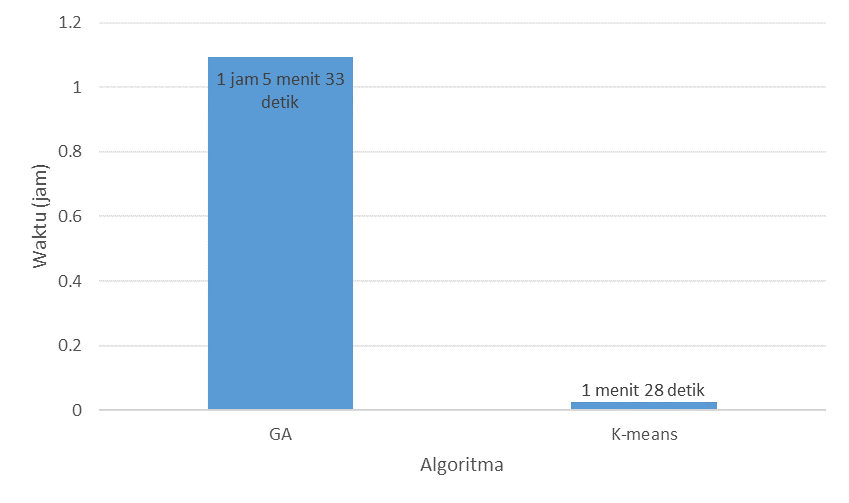
\includegraphics[width=0.6 \textwidth]{Grafik-kmeans-waktu}
	\caption{Grafik hubungan algoritma dengan waktu tempuh}
	\label{fig:graph:kmeans-time}
\end{figure}

Berdasarkan grafik pada Gambar \ref{fig:graph:kmeans-time}, waktu yang dibutuhkan algoritma genetika lebih banyak sekitar 4365\% dibandingkan dengan algoritma \textit{K-means}. Hal ini dikarenakan proses komputasi yang dilakukan pada algoritma genetika jauh lebih banyak dan kompleks dibandingkan dengan algoritma \textit{K-means}.

\begin{figure}[H]
	\centering
	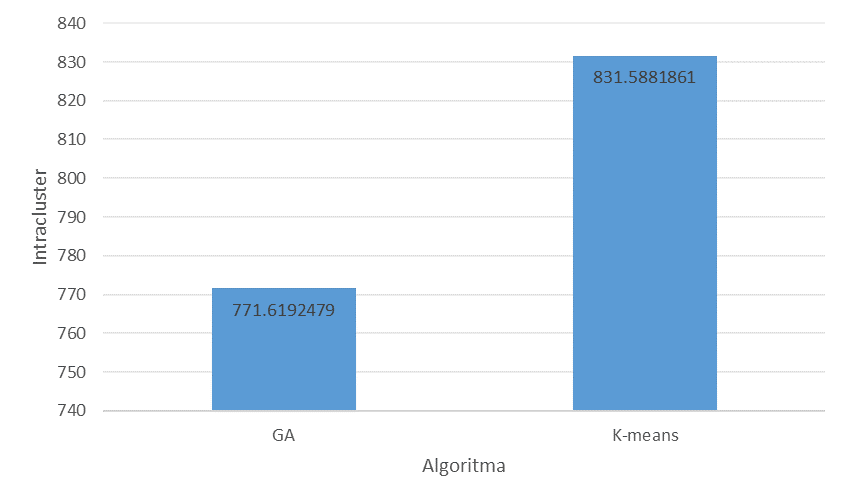
\includegraphics[width=0.6 \textwidth]{Grafik-kmeans-intracluster}
	\caption{Grafik hubungan algoritma dengan \textit{intracluster similarity}}
	\label{fig:graph:kmeans-intra}
\end{figure}

Berdasarkan grafik pada Gambar \ref{fig:graph:kmeans-intra}, nilai \textit{intracluster similarity} pada algoritma \textit{K-means} lebih besar 7\% daripada algoritma genetika.

\begin{figure}[H]
	\centering
	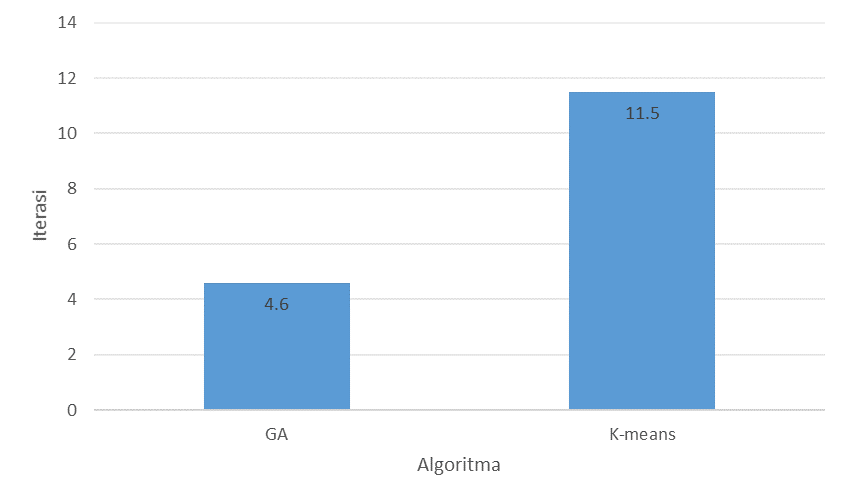
\includegraphics[width=0.6 \textwidth]{Grafik-kmeans-iterasi}
	\caption{Grafik hubungan algoritma dengan banyaknya iterasi}
	\label{fig:graph:kmeans-iteration}
\end{figure}

Berdasarkan grafik pada Gambar \ref{fig:graph:kmeans-iteration}, jumlah iterasi dengan menggunakan algoritma \textit{K-means} lebih banyak 150\% daripada algoritma genetika. Namun berdasarkan grafik pada Gambar \ref{fig:graph:kmeans-time}, waktu yang ditempuh \textit{K-means} lebih sebentar dibandingkan dengan algoritma genetika. Hal ini terjadi karena waktu yang diperlukan untuk menempuh satu iterasi pada \textit{K-means} jauh lebih kecil dibandingkan dengan waktu yang diperlukan untuk menempuh satu iterasi pada algoritma genetika.

\begin{figure}[H]
	\centering
	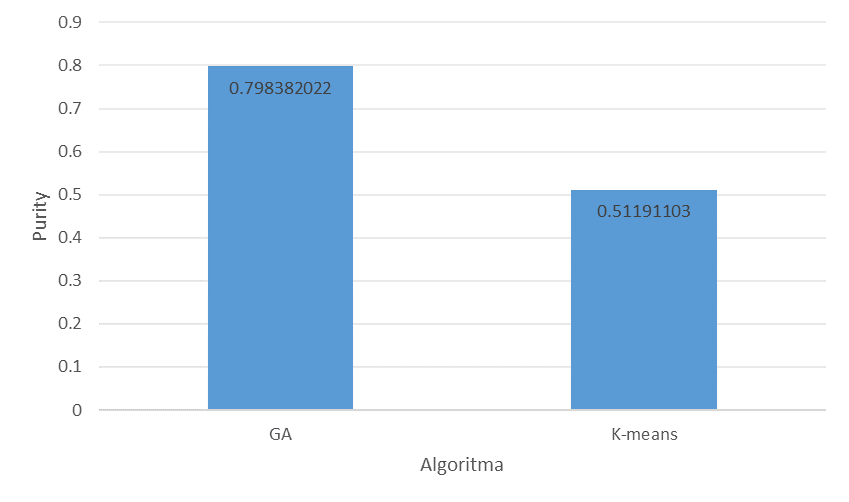
\includegraphics[width=0.6 \textwidth]{Grafik-kmeans-purity}
	\caption{Grafik hubungan algoritma dengan nilai \textit{purity}}
	\label{fig:graph:kmeans-purity}
\end{figure}

Berdasarkan grafik pada Gambar \ref{fig:graph:kmeans-purity}, nilai \textit{purity} algoritma genetika lebih besar 56\% dibandingkan dengan nilai \textit{purity} menggunakan algoritma \textit{K-means}.

\section{Kesimpulan Eksperimen}
Berdasarkan eksperimen yang telah dilakukan, dapat diambil beberapa kesimpulan sebagai berikut:

\begin{enumerate}
	\item Nilai \textit{purity} dan \textit{intracluster similarity} sama sekali tidak berhubungan. Padahal seharusnya semakin besar nilai \textit{intracluster similarity}, maka hasil pengelompokan akan semakin baik. Apabila hasil pengelompokan semakin baik, maka nilai \textit{purity} seharusnya semakin besar pula. Berdasarkan hasil eksperimen, nilai \textit{purity} lebih akurat dalam menentukan baik atau buruknya hasil suatu pengelompokan karena menggunakan label yang telah ada sebelumnya untuk mengukur kemurnian hasil pengelompokan. Dapat disimpulkan bahwa \textit{intracluster similarity} kurang merepresentasikan seberapa baik suatu hasil pengelompokan.
	\item Algoritma genetika lebih baik 56\% menurut nilai \textit{purity} (Gambar \ref{fig:graph:kmeans-purity}). Namun, kekurangan dari algoritma genetika adalah waktu pemrosesan yang jauh lebih lama dibandingkan dengan algoritma \textit{K-means}. 
	\item Berdasarkan hasil eksperimen dengan menggunakan algoritma \textit{K-means} (Tabel \ref{tbl:resKM} pada Lampiran \ref{lamp:B}), algoritma \textit{K-means} memang seringkali terjebak pada \textit{local optimum}. Hal ini dibuktikan dengan nilai \textit{purity} yang memiliki perbedaan cukup jauh antara satu dengan yang lainnya. Hasil dengan nilai \textit{purity} yang cukup kecil (misalkan pada baris ke-3 Tabel \ref{tbl:resKM} dengan nilai \textit{purity} 0.252080274 atau pada baris ke-10 Tabel \ref{tbl:resKM} dengan nilai \textit{purity} 0.248153619) merupakan contoh \textit{local optimum} yang dialami oleh \textit{K-means}.
	\item Berdasarkan hasil eksperimen menggunakan kasus uji 1 (Tabel \ref{tbl:res1} pada Lampiran \ref{lamp:B}). Nilai \textit{purity} pada hasil percobaan ini lebih stabil (memiliki rentang nilai yang kecil) dibandingkan dengan menggunakan algoritma \textit{K-means}. Dari lima kali pengujian, tidak ada satupun yang memiliki nilai \textit{purity} jauh dari rata-rata sehingga dapat disimpulkan bahwa algoritma genetika terbukti lebih baik dalam mengatasi \textit{local optimum}.
\end{enumerate}